%% ============================================================================
%% som_pipeline.tex -- README overview figure, som-multimodal-datareduction
%%
%% Purpose : one-row pipeline overview: multimodal measurements in, a trained
%%           self-organizing map (SOM), k-means clustering of the SOM codebook,
%%           and the interpretable maps out, with the command that runs each step.
%%           Same visual language as the sister figures (grey page, gold icon
%%           rings, navy stage boxes, grey phase brackets).
%% Build   : (from docs/figures/src/)
%%           pdflatex som_pipeline.tex
%%           pdftoppm -png -r 254 -singlefile som_pipeline.pdf ../som_pipeline
%%           cp som_pipeline.pdf ../../som_pipeline.pdf
%% Output  : a 26.6 cm x 10 cm vector PDF (~2660 px PNG at 254 dpi); at GitHub's
%%           ~830-1000 px display width the 16 pt box labels land near 16-19 px.
%% Layout  : fixed y-bands and x-centres, as in the sister figures, so text never
%%           overlaps an icon; each caption opens with the file or command for that step.
%% ============================================================================
\documentclass[tikz,border=0pt]{standalone}
\usepackage[T1]{fontenc}
\usepackage{lmodern}                      % scalable tt/math fonts (no bitmap substitutions)
\usepackage[scaled=0.95]{helvet}          % Helvetica metrics, like the sister figures
\renewcommand{\familydefault}{\sfdefault}
\usepackage[letterspace=80]{microtype}   % \textls: tracked capitals for phase labels
\usetikzlibrary{arrows.meta,calc}
\pdfinfo{/Title (som-multimodal-datareduction: pipeline overview) /Author (Cameron B. Renteria)}

% ---- palette (identical to the sister figures) ---------------------------------------------
\definecolor{page}{HTML}{EEEEEE}    % page grey
\definecolor{navy}{HTML}{1E3252}    % stage boxes, line icons, arrows
\definecolor{gold}{HTML}{B8894A}    % icon rings, highlights
\definecolor{ink}{HTML}{222222}     % caption text
\definecolor{phase}{HTML}{6E6E6A}   % phase labels
\definecolor{rule}{HTML}{8C8C8C}    % phase brackets
\definecolor{tone}{HTML}{C9CED6}    % neutral fill inside icons
\definecolor{sky}{HTML}{7F9BBF}     % mid tone for heat-map icons

% ---- reusable styles ----------------------------------------------------------------------
\tikzset{
  stage/.style = {fill=navy, rounded corners=6pt, minimum width=4.6cm, minimum height=1.75cm,
                  text=white, align=center, font=\fontsize{16}{18.5}\selectfont, inner sep=2pt},
  ring/.style  = {draw=gold, line width=1.6pt, circle, minimum size=2.2cm},
  capt/.style  = {text=ink, align=center, anchor=north, text width=6.3cm,
                  font=\fontsize{12}{14.5}\selectfont},
  flow/.style  = {-{Stealth[length=7pt,width=6.5pt]}, line width=1.4pt, draw=navy},
  ico/.style   = {draw=navy, line width=1.1pt},
  phaselbl/.style = {text=phase, font=\fontsize{11.5}{13.5}\selectfont},
}
% Command / file names in captions: gold, bold typewriter.
\newcommand{\cmdfont}{\color{gold}\ttfamily\bfseries\fontsize{11.5}{13.5}\selectfont}
% Phase bracket: grey rule with short down-ticks from x=#1 to x=#2, label #3 centred above.
\newcommand{\phasebracket}[3]{%
  \draw[rule, line width=1pt] (#1,8.35) -- (#1,8.6) -- (#2,8.6) -- (#2,8.35);
  \node[phaselbl] at ({(#1+#2)/2},9.1) {\textls{#3}};}

\begin{document}
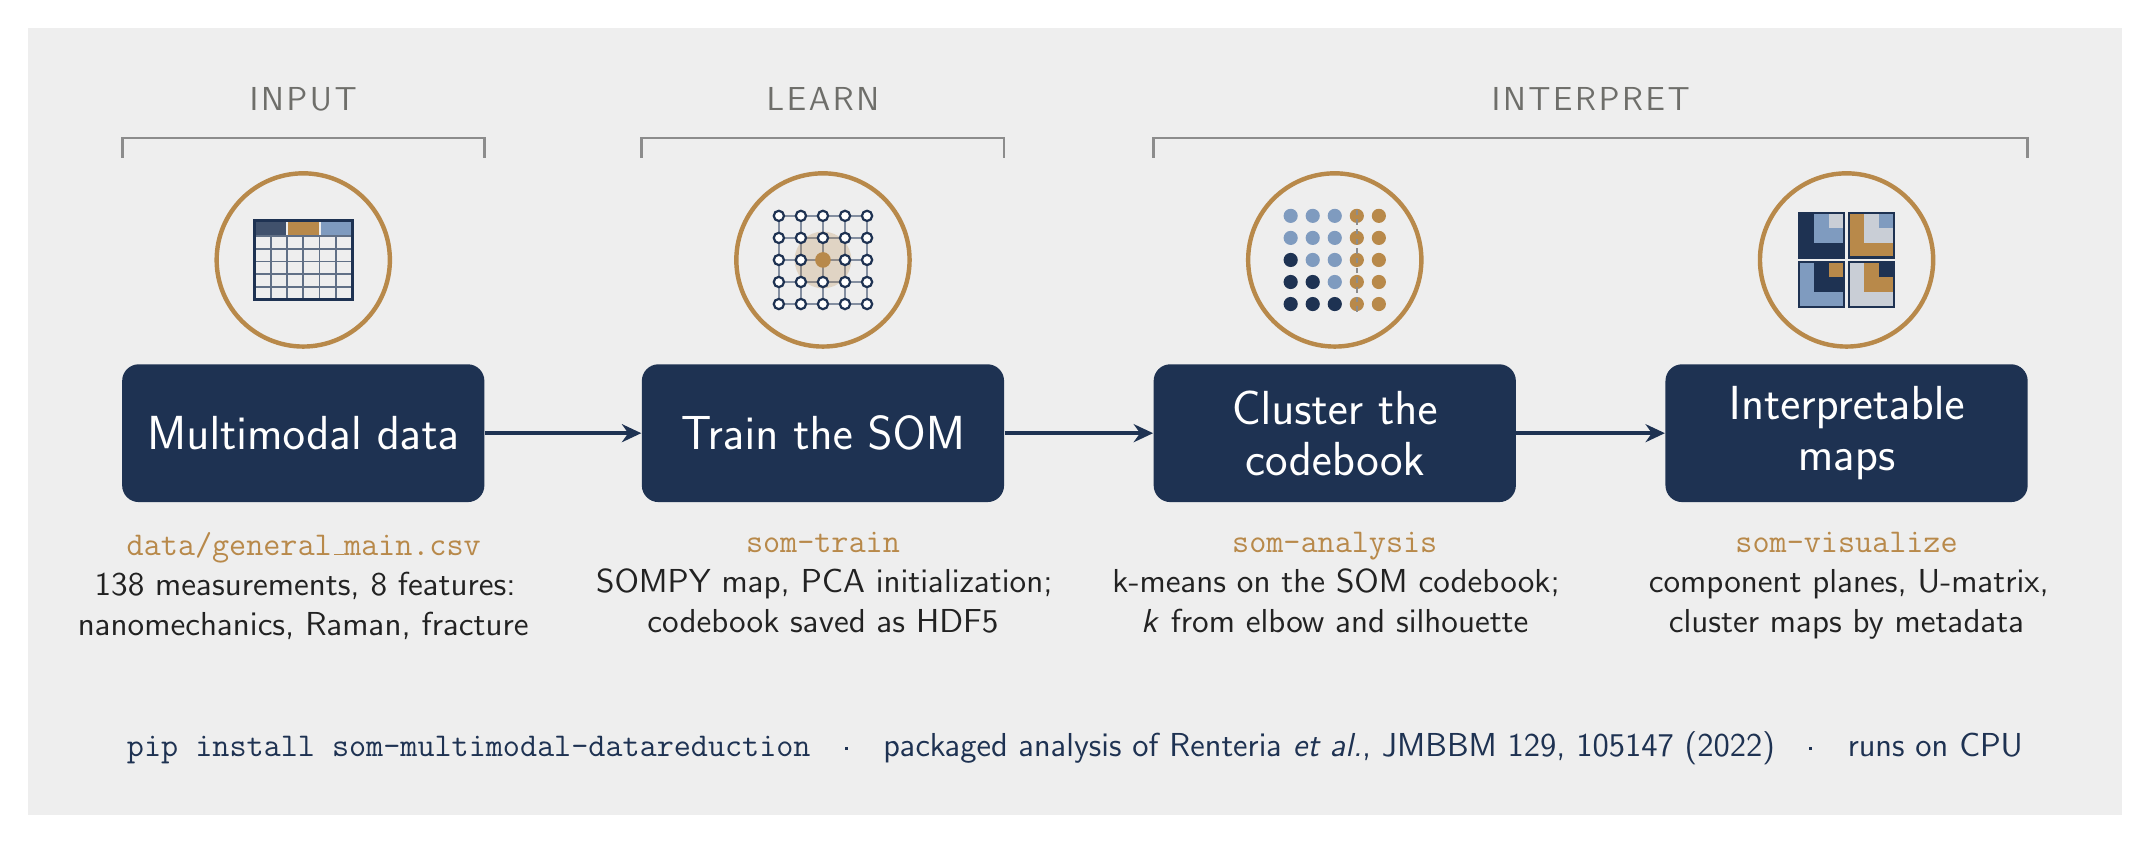
\begin{tikzpicture}[x=1cm,y=1cm]

% ---- page -------------------------------------------------------------------------------
\fill[page] (0,0) rectangle (26.6,10);

% ---- column centres (x) and fixed row bands (y) -------------------------------------------
%  data 3.5 | train 10.1 | cluster 16.6 | maps 23.1   (6.5-6.6 cm pitch, 4.6 cm boxes)
\def\yring{7.05}   % icon ring centres
\def\ybox{4.85}    % stage box centres
\def\ycap{3.72}    % caption tops

% ---- phase brackets -----------------------------------------------------------------------
\phasebracket{1.2}{5.8}{INPUT}
\phasebracket{7.8}{12.4}{LEARN}
\phasebracket{14.3}{25.4}{INTERPRET}

% ---- icon rings -----------------------------------------------------------------------------
\foreach \x in {3.5,10.1,16.6,23.1} \node[ring] at (\x,\yring) {};

% Icon 1 -- multimodal table: rows = specimens, column blocks = measurement families.
\begin{scope}[shift={(3.5,\yring)}]
  \fill[navy!85] (-0.62,0.30) rectangle (-0.22,0.50);
  \fill[gold]    (-0.20,0.30) rectangle ( 0.20,0.50);
  \fill[sky]     ( 0.22,0.30) rectangle ( 0.62,0.50);
  \foreach \j in {0,...,4} \foreach \i in {0,...,5}
    \draw[navy!70, line width=0.6pt] ({-0.62+\i*0.2067},{0.30-(\j+1)*0.16}) rectangle ++(0.2067,0.16);
  \draw[ico] (-0.62,-0.50) rectangle (0.62,0.50);
\end{scope}

% Icon 2 -- SOM training: node lattice; best-matching unit (gold) and its neighbourhood.
\begin{scope}[shift={(10.1,\yring)}]
  \foreach \i in {0,...,4} {
    \draw[navy!55, line width=0.6pt] ({-0.56+\i*0.28},-0.56) -- ({-0.56+\i*0.28},0.56);
    \draw[navy!55, line width=0.6pt] (-0.56,{-0.56+\i*0.28}) -- (0.56,{-0.56+\i*0.28}); }
  \fill[gold, opacity=0.25] (0,0) circle (0.36);
  \foreach \i in {0,...,4} \foreach \j in {0,...,4}
    \filldraw[navy, fill=white, line width=0.8pt] ({-0.56+\i*0.28},{-0.56+\j*0.28}) circle (0.065);
  \filldraw[gold, line width=0.8pt] (0,0) circle (0.085);
\end{scope}

% Icon 3 -- clustering the codebook: the same lattice, nodes coloured by three k-means groups.
\begin{scope}[shift={(16.6,\yring)}]
  \foreach \i in {0,...,4} \foreach \j in {0,...,4} {
    \pgfmathtruncatemacro{\g}{(\i+\j<3) ? 0 : ((\i>2) ? 1 : 2)}  % cluster id 0/1/2
    \ifnum\g=0 \def\cc{navy}\fi \ifnum\g=1 \def\cc{gold}\fi \ifnum\g=2 \def\cc{sky}\fi
    \fill[\cc] ({-0.56+\i*0.28},{-0.56+\j*0.28}) circle (0.09); }
  \draw[rule, line width=0.8pt, dash pattern=on 2pt off 1.5pt] (0.28,-0.66) -- (0.28,0.66);
\end{scope}

% Icon 4 -- interpretable maps: a 2 x 2 panel of component-plane heat maps.
\begin{scope}[shift={(23.1,\yring)}]
  \foreach \px/\py/\a/\b/\c in {-0.6/0.03/navy/sky/tone, 0.03/0.03/gold/tone/sky,
                                 -0.6/-0.6/sky/navy/gold, 0.03/-0.6/tone/gold/navy} {
    \fill[\a] (\px,\py) rectangle ++(0.57,0.57);
    \fill[\b] (\px+0.19,\py+0.19) rectangle ++(0.38,0.38);
    \fill[\c] (\px+0.38,\py+0.38) rectangle ++(0.19,0.19);
    \draw[navy, line width=0.8pt] (\px,\py) rectangle ++(0.57,0.57); }
\end{scope}

% ---- stage boxes ------------------------------------------------------------------------------
\node[stage] (dat) at (3.5,\ybox)  {Multimodal data};
\node[stage] (trn) at (10.1,\ybox) {Train the SOM};
\node[stage] (cls) at (16.6,\ybox) {Cluster the\\codebook};
\node[stage] (map) at (23.1,\ybox) {Interpretable\\maps};

% ---- flow arrows ------------------------------------------------------------------------------
\draw[flow] (dat.east) -- (trn.west);
\draw[flow] (trn.east) -- (cls.west);
\draw[flow] (cls.east) -- (map.west);

% ---- captions: the command first (gold), then what the step does ------------------------------
\node[capt] at (3.5,\ycap)  {{\cmdfont data/general\_main.csv}\\138 measurements, 8 features:\\nanomechanics, Raman, fracture};
\node[capt] at (10.1,\ycap) {{\cmdfont som-train}\\SOMPY map, PCA initialization;\\codebook saved as HDF5};
\node[capt] at (16.6,\ycap) {{\cmdfont som-analysis}\\k-means on the SOM codebook;\\\textit{k} from elbow and silhouette};
\node[capt] at (23.1,\ycap) {{\cmdfont som-visualize}\\component planes, U-matrix,\\cluster maps by metadata};

% ---- footer ---------------------------------------------------------------------------------------
\node[text=navy, font=\fontsize{12}{14.5}\selectfont] at (13.3,0.85)
  {\texttt{pip install som-multimodal-datareduction}\quad\textperiodcentered\quad
   packaged analysis of Renteria \textit{et al.}, JMBBM 129, 105147 (2022)\quad\textperiodcentered\quad runs on CPU};

\end{tikzpicture}
\end{document}
